\documentclass{article}
\usepackage[spanish]{babel}
\usepackage[utf8]{inputenc}
\usepackage[T1]{fontenc}
\usepackage{graphicx}
\usepackage[numbers,sort&compress]{natbib}

\title{\bf Práctica 1: movimiento Browniano}
\date{\today}
\author{C. A. Estrada}

\begin{document}

\maketitle

\section{Objetivo}
Observar sistemáticamente el efecto de la dimensión en el tiempo de regreso al origen de una partícula en el movimiento Browniano \cite{dra}, para dimensiones 1 a 8, variando el número de pasos de la caminata en potencias de dos con exponentes de 5 a 10, realizando 50 repeticiones de cada experimento.

\section{Metodología}
Para efectos de esta práctica, se utilizó el paquete estadístico R versión 4.0.2 \cite{R}. Se generó un código que evalúe el tiempo de regreso al origen en pasos, tomando como base códigos previamente registrados: una rutina para la caminata de la partícula \cite{dra}, así como una rutina tipo loop de ``for'' anidada \cite{codigo}. Se tomó en cuenta que el tiempo se discretizó en ``pasos'' dentro de la caminata, con iguales probabilidades de dirigir un paso hacia la drecha o la izquierda desde el origen.

El número de pasos (largo de la caminata) fue variado como potencias de dos con exponentes de 5 a 10, variando las dimensiones de 1 a 8, programando 50 repeticiones para cada experimento. Finalmente, se realizó un gráfico de caja-bigote de los resultados obtenidos del tiempo de regreso al origen en función de las dimensiones.  

\section{Resultados y discusión}
El número de dimensiones se aumentó de manera lineal de 1 hasta 8, para observar su efecto en el tiempo de regreso al origen de una partícula hipotética, como se observa en la figura \ref{figura1}.
\begin{figure}[ptb]
\begin{center}
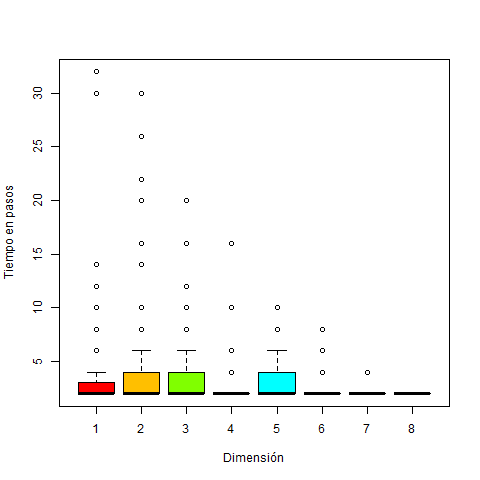
\includegraphics[width=\linewidth]{Practica1.png}
\end{center}
\caption{Tiempo de regreso al origen (en pasos) en función del número de dimensiones.\label{figura1}}
\end{figure}
Para una sola dimensión, se presentaron varias anomalías, siendo 32 el número máximo de pasos obtenidos, aunque en la mayoría de las repeticiones fueron 2 pasos. Con dos dimensiones, el número de pasos más frecuente fue de 4, con varias anomalías, y el tiempo máximo para esta dimensión fue de 30 pasos. En tres y cinco dimensiones, los resultados fueron bastante similares que con dos dimensiones, pero la cantidad de anomalías disminuyó, siendo 20 y 10 el número de pasos máximo obtenido, respectivamente. 

Para las dimensiones cuatro, seis, siete y ocho, la cantidad de repeticiones que regresan al origen dismuniyó en gran manera, siendo 2 el número de pasos de tiempo de regreso al origen más frecuente; a su vez, se observa una disminución progresiva del tiempo de regreso al origen en el número máximo (representado por la anomalía máxima en el gráfico) conforme se aumenta la cantidad de dimensiones, que para el caso de ocho dimensiones sería de 2 pasos. Respecto a frecuencia del tiempo en pasos según la dimensión, debido a la naturaleza pseudoaleatoria de la prueba, no se observa una tendencia clara para el número de dimensiones intermedio (dimensiones cuatro y cinco), salvo que para el resto de la dimensiones, entre menor sea el número de dimensiones, mayor es el tiempo de regreso al origen y existe una mayor cantidad de repeticiones. Por ende, puede inferirse que a mayor cantidad de dimensiones, la mayoría de los resultados del experimento no regresan al origen.

\section{Conclusión}
Entre menor sea la cantidad de dimensiones, mayor es el tiempo de regreso al origen.

\bibliography{P1}
\bibliographystyle{unsrtnat}

\end{document}
